\documentclass{article}

%%%%%%%%%%%%%%%%%%%%%%%%%%%%%%%%%%%%%%%%%
% Lachaise Assignment
% Structure Specification File
% Version 1.0 (26/6/2018)
%
% This template originates from:
% http://www.LaTeXTemplates.com
%
% Authors:
% Marion Lachaise & François Févotte
% Vel (vel@LaTeXTemplates.com)
%
% License:
% CC BY-NC-SA 3.0 (http://creativecommons.org/licenses/by-nc-sa/3.0/)
% 
%%%%%%%%%%%%%%%%%%%%%%%%%%%%%%%%%%%%%%%%%

%----------------------------------------------------------------------------------------
%	PACKAGES AND OTHER DOCUMENT CONFIGURATIONS
%----------------------------------------------------------------------------------------

\usepackage{amsmath,amsfonts,stmaryrd,amssymb} % Math packages

\usepackage{enumerate} % Custom item numbers for enumerations

\usepackage[ruled]{algorithm2e} % Algorithms

\usepackage[framemethod=tikz]{mdframed} % Allows defining custom boxed/framed environments

\usepackage{listings} % File listings, with syntax highlighting
\lstset{
	basicstyle=\ttfamily, % Typeset listings in monospace font
}

%----------------------------------------------------------------------------------------
%	DOCUMENT MARGINS
%----------------------------------------------------------------------------------------

\usepackage{geometry} % Required for adjusting page dimensions and margins

\geometry{
	paper=a4paper, % Paper size, change to letterpaper for US letter size
	top=2.5cm, % Top margin
	bottom=3cm, % Bottom margin
	left=2.5cm, % Left margin
	right=2.5cm, % Right margin
	headheight=14pt, % Header height
	footskip=1.5cm, % Space from the bottom margin to the baseline of the footer
	headsep=1.2cm, % Space from the top margin to the baseline of the header
	%showframe, % Uncomment to show how the type block is set on the page
}

%----------------------------------------------------------------------------------------
%	FONTS
%----------------------------------------------------------------------------------------

\usepackage[utf8]{inputenc} % Required for inputting international characters
\usepackage[T1]{fontenc} % Output font encoding for international characters

\usepackage{XCharter} % Use the XCharter fonts

%----------------------------------------------------------------------------------------
%	COMMAND LINE ENVIRONMENT
%----------------------------------------------------------------------------------------

% Usage:
% \begin{commandline}
%	\begin{verbatim}
%		$ ls
%		
%		Applications	Desktop	...
%	\end{verbatim}
% \end{commandline}

\mdfdefinestyle{commandline}{
	leftmargin=10pt,
	rightmargin=10pt,
	innerleftmargin=15pt,
	middlelinecolor=black!50!white,
	middlelinewidth=2pt,
	frametitlerule=false,
	backgroundcolor=black!5!white,
	frametitle={Command Line},
	frametitlefont={\normalfont\sffamily\color{white}\hspace{-1em}},
	frametitlebackgroundcolor=black!50!white,
	nobreak,
}

% Define a custom environment for command-line snapshots
\newenvironment{commandline}{
	\medskip
	\begin{mdframed}[style=commandline]
}{
	\end{mdframed}
	\medskip
}

%----------------------------------------------------------------------------------------
%	FILE CONTENTS ENVIRONMENT
%----------------------------------------------------------------------------------------

% Usage:
% \begin{file}[optional filename, defaults to "File"]
%	File contents, for example, with a listings environment
% \end{file}

\mdfdefinestyle{file}{
	innertopmargin=1.6\baselineskip,
	innerbottommargin=0.8\baselineskip,
	topline=false, bottomline=false,
	leftline=false, rightline=false,
	leftmargin=2cm,
	rightmargin=2cm,
	singleextra={%
		\draw[fill=black!10!white](P)++(0,-1.2em)rectangle(P-|O);
		\node[anchor=north west]
		at(P-|O){\ttfamily\mdfilename};
		%
		\def\l{3em}
		\draw(O-|P)++(-\l,0)--++(\l,\l)--(P)--(P-|O)--(O)--cycle;
		\draw(O-|P)++(-\l,0)--++(0,\l)--++(\l,0);
	},
	nobreak,
}

% Define a custom environment for file contents
\newenvironment{file}[1][File]{ % Set the default filename to "File"
	\medskip
	\newcommand{\mdfilename}{#1}
	\begin{mdframed}[style=file]
}{
	\end{mdframed}
	\medskip
}

%----------------------------------------------------------------------------------------
%	NUMBERED QUESTIONS ENVIRONMENT
%----------------------------------------------------------------------------------------

% Usage:
% \begin{question}[optional title]
%	Question contents
% \end{question}

\mdfdefinestyle{question}{
	innertopmargin=1.2\baselineskip,
	innerbottommargin=0.8\baselineskip,
	roundcorner=5pt,
	nobreak,
	singleextra={%
		\draw(P-|O)node[xshift=1em,anchor=west,fill=white,draw,rounded corners=5pt]{%
		Question \theQuestion\questionTitle};
	},
}

\newcounter{Question} % Stores the current question number that gets iterated with each new question

% Define a custom environment for numbered questions
\newenvironment{question}[1][\unskip]{
	\bigskip
	\stepcounter{Question}
	\newcommand{\questionTitle}{~#1}
	\begin{mdframed}[style=question]
}{
	\end{mdframed}
	\medskip
}

%----------------------------------------------------------------------------------------
%	WARNING TEXT ENVIRONMENT
%----------------------------------------------------------------------------------------

% Usage:
% \begin{warn}[optional title, defaults to "Warning:"]
%	Contents
% \end{warn}

\mdfdefinestyle{warning}{
	topline=false, bottomline=false,
	leftline=false, rightline=false,
	nobreak,
	singleextra={%
		\draw(P-|O)++(-0.5em,0)node(tmp1){};
		\draw(P-|O)++(0.5em,0)node(tmp2){};
		\fill[black,rotate around={45:(P-|O)}](tmp1)rectangle(tmp2);
		\node at(P-|O){\color{white}\scriptsize\bf !};
		\draw[very thick](P-|O)++(0,-1em)--(O);%--(O-|P);
	}
}

% Define a custom environment for warning text
\newenvironment{warn}[1][Warning:]{ % Set the default warning to "Warning:"
	\medskip
	\begin{mdframed}[style=warning]
		\noindent{\textbf{#1}}
}{
	\end{mdframed}
}

%----------------------------------------------------------------------------------------
%	INFORMATION ENVIRONMENT
%----------------------------------------------------------------------------------------

% Usage:
% \begin{info}[optional title, defaults to "Info:"]
% 	contents
% 	\end{info}

\mdfdefinestyle{info}{%
	topline=false, bottomline=false,
	leftline=false, rightline=false,
	nobreak,
	singleextra={%
		\fill[black](P-|O)circle[radius=0.4em];
		\node at(P-|O){\color{white}\scriptsize\bf i};
		\draw[very thick](P-|O)++(0,-0.8em)--(O);%--(O-|P);
	}
}

% Define a custom environment for information
\newenvironment{info}[1][Info:]{ % Set the default title to "Info:"
	\medskip
	\begin{mdframed}[style=info]
		\noindent{\textbf{#1}}
}{
	\end{mdframed}
}
 % Include the file specifying the document structure and custom commands

\usepackage{graphicx}
\usepackage{float}
\usepackage{caption}
\renewcommand{\thealgocf}{} % Stop numbering in header of algorithms
\SetKwRepeat{Do}{do}{while} % Do while loop for algorithms

%----------------------------------------------------------------------------------------
%	ASSIGNMENT INFORMATION
%----------------------------------------------------------------------------------------

\title{EELE465 Lab 0} % Title of the assignment

\author{Ryan French\\ \texttt{ryanfrench3@montana.edu}} % Author name and email address

\date{Montana State University --- \today} % University, school and/or department name(s) and a date

%----------------------------------------------------------------------------------------

\begin{document}
\maketitle % Print the title

%----------------------------------------------------------------------------------------
%	INTRODUCTION
%----------------------------------------------------------------------------------------

\section*{Introduction}

The MSP430FR2355 LaunchPad\texttrademark Development Kit contains two on-board LEDs which are useful for monitoring the progression of code. In this lab, one of these LEDs was used a "heartbeat indicator": a constantly-flashing signal that implies an active microcontroller. To achieve the given frequency of 0.5 Hz, three methods were implemented: a register-decrement loop, an internal timing interrupt, and a combination of the two methods (flow charts for each of these methods can be found in the appendix). This resulted in subroutines that will be useful in the future, when more complicated firmware is written to the board.


%\begin{info} % Information block
%	This is an interesting piece of information, to which the reader should pay special attention. Fusce varius orci ac magna dapibus porttitor. In tempor leo a neque bibendum sollicitudin. Nulla pretium fermentum nisi, eget sodales magna facilisis eu. Praesent aliquet nulla ut bibendum lacinia. Donec vel mauris vulputate, commodo ligula ut, egestas orci. Suspendisse commodo odio sed hendrerit lobortis. Donec finibus eros erat, vel ornare enim mattis et.
%\end{info}
%----------------------------------------------------------------------------------------


%----------------------------------------------------------------------------------------
%	SETUP
%----------------------------------------------------------------------------------------

\section*{Setup}

Since the LaunchPad comes fully assembled, there was no need to manually set up a circuit for the microcontroller. The MCU is flashed by a USB cable connected to a computer running Code Composer Studio. CCS is an IDE created by Texas Instruments, designed specifically for their microcontrollers. It features an integrated debugger and builder/flasher.

%----------------------------------------------------------------------------------------


% Numbered question, with subquestions in an enumerate environment
%\begin{question}
%	Quisque ullamcorper placerat ipsum. Cras nibh. Morbi vel justo vitae lacus tincidunt ultrices. Lorem ipsum dolor sit amet, consectetuer adipiscing elit.
%
%	% Subquestions numbered with letters
%	\begin{enumerate}[(a)]
%		\item Do this.
%		\item Do that.
%		\item Do something else.
%	\end{enumerate}
%\end{question}
%	
%------------------------------------------------


%----------------------------------------------------------------------------------------
%	SOLUTION 1
%----------------------------------------------------------------------------------------

\section*{Solution 1:  Decrement Loop}

To implement this solution, it was necessary to figure out how long it took the counter decrement subroutine to complete. Several initial values were used and their frequencies recorded. These values were plotted and subjected to a cubic spline interpolation algorithm to find a factor of 0.5 Hz. This value was placed in the register for decrementing and the decrement subroutine was looped over N times, where N is the quotient of the aforementioned factor and desired frequency.

%\subsection*{Algorithm}

\begin{center}
	\begin{minipage}{0.6\linewidth} % Adjust the minipage width to accomodate for the length of algorithm lines
		\begin{algorithm}[H]
			\KwIn{$(N, DEC)$:  Number of Loops, Decrement Initial Value}  % Algorithm inputs
			%\KwResult{$(c, d)$, such that $a+b = c + d$} % Algorithm outputs/results
			\medskip
			set LED \;
			\While {True}{
			$n= N$ \;
			\While{$n \neq 0$}{
			$dec = DEC$ \;
			\While{$dec \neq 0$}{
				$dec = dec - 1$ \;
			}
				$n = n - 1$ \;
			}
			toggle LED \;
			}
			\caption{Decrement Loop} % Algorithm name
			\label{alg:DecLoop}   % optional label to refer to
		\end{algorithm}
	\end{minipage}
\end{center}

%----------------------------------------------------------------------------------------

%% Numbered question, with an optional title
%\begin{question}[\itshape (with optional title)]
%
%\end{question}


%----------------------------------------------------------------------------------------
%	SOLUTION 2
%----------------------------------------------------------------------------------------

\section*{Solution 2:  Timer Interrupt}

This solution relies on one of the internal timers of the microcontroller. Initializing the MCU involves enabling the timer overflow interrupt (as well as other setup instructions). Running the code with a prescalar value of 1 reveals the base frequency of the timer overflow interrupt. This value could then be altered to output a frequency of 0.5 Hz (prescalar = 8).

%\subsection*{Algorithm}

\begin{center}
	\begin{minipage}{0.6\linewidth} % Adjust the minipage width to accomodate for the length of algorithm lines
		\begin{algorithm}[H]
			\KwIn{N/A}  % Algorithm inputs
			%\KwResult{$(c, d)$, such that $a+b = c + d$} % Algorithm outputs/results
			\medskip
			set LED \;
			\While {True}{
			\If{interrupt}{
			toggle LED \;
			}
			}
			\caption{Timer Interrupt} % Algorithm name
			\label{alg:Int}   % optional label to refer to
		\end{algorithm}
	\end{minipage}
\end{center}

%----------------------------------------------------------------------------------------



%----------------------------------------------------------------------------------------
%	SOLUTION 3
%----------------------------------------------------------------------------------------

\section*{Solution 3:  Decrement and Interrupt}

Here, a combination of the previous two methods was used to create a highly-accurate frequency. For this, the prescalar value for the timer was set to 1. This method was implemented by first waiting for a timer interrupt and looping over a decrement subroutine inside the interrupt before returning from the interrupt. To achieve the needed frequency, first a number of loops was chosen ($N = 20$). Then, similar to solution 1, decrement values were plotted against frequencies and a cubic spline interpolation was used to find the optimal value for the initial decrement variable. This method led to a frequency within 0.1\% of 0.5 Hz.

%\subsection*{Algorithm}

\begin{center}
	\begin{minipage}{0.6\linewidth} % Adjust the minipage width to accomodate for the length of algorithm lines
		\begin{algorithm}[H]
			\KwIn{$(N, DEC)$: Number of Loops, Decrement Initial Value}  % Algorithm inputs
			%\KwResult{$(c, d)$, such that $a+b = c + d$} % Algorithm outputs/results
			\medskip
			set LED \;
			\While {True}{
			\If{interrupt}{
			$n = N$ \;
			\While{$n \neq 0$}{
			$dec = DEC$ \;
			\While{$dec \neq 0$}{
			$dec = dec - 1$ \;
			}
			$n = n - 1$ \;			
			}
			toggle LED \;
			}
			}
			\caption{Decrement and Interrupt} % Algorithm name
			\label{alg:DecInt}   % optional label to refer to
		\end{algorithm}
	\end{minipage}
\end{center}

%----------------------------------------------------------------------------------------



%----------------------------------------------------------------------------------------
%	COMMENTS
%----------------------------------------------------------------------------------------
\section*{Comments}

The main hurdle encountered in this lab was learning the assembly instructions for this microcontroller, and a lot of time was spent reading through the header files looking for the defined constants (especially when setting up the timer). Another issue was determining the initial decrement value, because there is a turnover once a certain number is used (i.e., increasing the value beyond a certain value caused a discontinuity in the frequency). Once it was decided to interpolate the data, it was easy to find this value.

%----------------------------------------------------------------------------------------



%----------------------------------------------------------------------------------------
%	Implementation
%----------------------------------------------------------------------------------------

%\section{Implementation}
%
%% File contents
%\begin{file}[hello.py]
%\begin{lstlisting}[language=Python]
%#! /usr/bin/python
%
%import sys
%sys.stdout.write("Hello World!\n")
%\end{lstlisting}
%\end{file}

%----------------------------------------------------------------------------------------

%% Command-line "screenshot"
%\begin{commandline}
%	\begin{verbatim}
%		$ chmod +x hello.py
%		$ ./hello.py
%
%		Hello World!
%	\end{verbatim}
%\end{commandline}

%% Warning text, with a custom title
%\begin{warn}[Notice:]
%  In congue risus leo, in gravida enim viverra id. Donec eros mauris, bibendum vel dui at, tempor commodo augue. In vel lobortis lacus. Nam ornare ullamcorper mauris vel molestie. Maecenas vehicula ornare turpis, vitae fringilla orci consectetur vel. Nam pulvinar justo nec neque egestas tristique. Donec ac dolor at libero congue varius sed vitae lectus. Donec et tristique nulla, sit amet scelerisque orci. Maecenas a vestibulum lectus, vitae gravida nulla. Proin eget volutpat orci. Morbi eu aliquet turpis. Vivamus molestie urna quis tempor tristique. Proin hendrerit sem nec tempor sollicitudin.
%\end{warn}

\pagebreak

\section*{Appendix}

\begin{centering}
\begin{figure}[H]
\label{system}
\centering
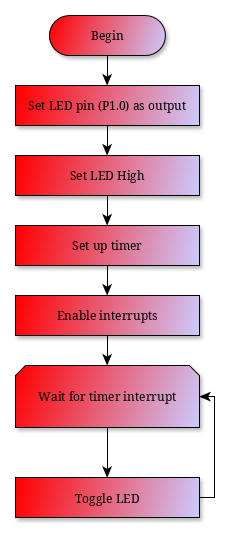
\includegraphics[width = 0.3\textwidth]{Lab0_part1.png}
\captionsetup{format = hang, width = 0.75\textwidth}
\caption{Decrement Loop Solution}
\label{fig:DecLoop}
\end{figure}
\end{centering}

\pagebreak

\begin{centering}
\begin{figure}[H]
\label{system}
\centering
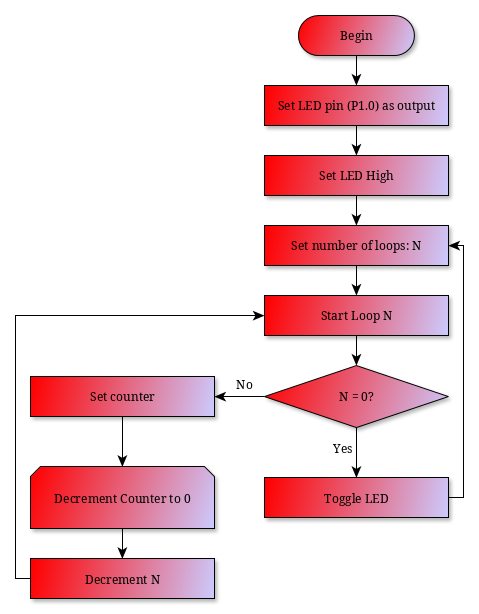
\includegraphics[width = 0.6\textwidth]{Lab0_part2.png}
\captionsetup{format = hang, width = 0.75\textwidth}
\caption{Timer Interrupt Solution}
\label{fig:Int}
\end{figure}
\end{centering}

\pagebreak

\begin{centering}
\begin{figure}[H]
\label{system}
\centering
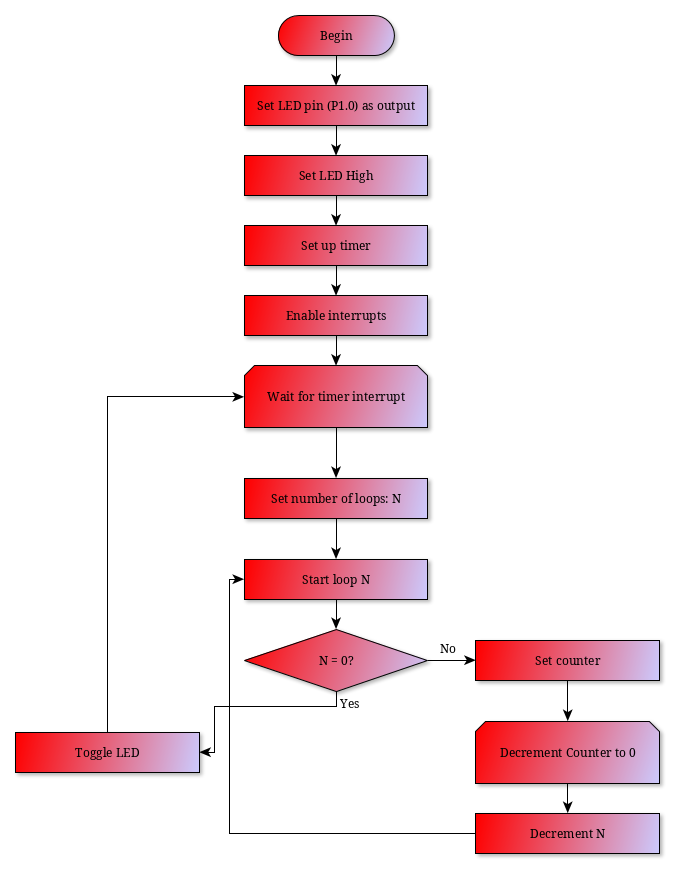
\includegraphics[width = 0.75\textwidth]{Lab0_part3.png}
\captionsetup{format = hang, width = 0.75\textwidth}
\caption{Combined Solution}
\label{fig:DecInt}
\end{figure}
\end{centering}



%----------------------------------------------------------------------------------------
%	END OF DOCUMENT
%----------------------------------------------------------------------------------------

\end{document}
